\documentclass[11pt,a4paper]{article}
% rozmery stranky
\usepackage[left=1.5cm,text={18cm, 25cm},top=2.5cm]{geometry}
% cestina a fonty
\usepackage[czech]{babel}
\usepackage[utf8]{inputenc}
\usepackage[T1]{fontenc}
% dalsi balicky
\usepackage{graphicx}
\usepackage{enumitem}
\usepackage{url}
\usepackage[bookmarksopen,colorlinks,plainpages=false,urlcolor=blue,
unicode,linkcolor=black]{hyperref}


\begin{document}

  \begin{titlepage}
    \begin{center}
      \Huge
      \textsc{Fakulta informačních technologií \\ Vysoké učení technické v~Brně}
      \vspace{100px}
      \begin{figure}[!h]
        \centering
        
\includegraphics[height=5cm]{logo}
      \end{figure}
      \\[50mm]
      \LARGE{Tvorba uživatelských rozhraní \,--\, projekt č. 93 \\
             Správa hostingu}
      \vfill
    \end{center}
    \Large{Roman Blanco (xblanc01) - kapitán týmu \hfill 24.10.2014 \\
           Adam Jež (xjezad00)}

  \end{titlepage}

  \section{Abstrakt}

    Cílem zadaného projektu je navrhnout a vytvořit uživatelské rozhraní,
    umožňující uživateli konfigurovat a spravovat své hostingové služby.
    Námi navržené rozhraní by mělo umožňovat správu FTP účtů, DNS
    záznamů, e-mailů a MySQL databází. Ovládání rozhraní navrhujeme tak, aby
    bylo přizpůsobeno jak uživatelům stolních počítačů, tak i uživatelům
    mobilních zařízení, které dokáží zobrazit internetový obsah. Protože naší
    snahou je maximální komfort zákazníků, nejčastěji užívané úkony by měly
    být lehce a rychle proveditelné.

  \section{Úvod}

    V~současnosti již existuje mnoho řešení uživatelských rozhraní pro správu
    hostingu.

    Při vyhledávání inspiračního materiálu jsme se zaměřili na vlastní práci s
    rozhraním - přehledost obsahu, způsob práce s daty a jejich řazení.
    Při návrhu vlastního rozhraní jsme se snažili vyvarovat případných chyb,
    které jsme nalézali v existujících řešeních. Z tohoto hlediska nám
    materiál poskytl jak pozitivní, tak i negativní inspiraci.  Jako studijní
    materiál nám sloužilo především rozhraní webhostingů roští.cz a wedos.cz \\
    \begin{figure}[ht]
      \begin{center}
        \includegraphics[width=12cm]{rosti}
        \caption{Uživatelské rozhraní webhostingu roští.cz}
      \end{center}
    \end{figure}
    \begin{figure}[ht]
      \begin{center}
        \includegraphics[width=12cm]{wedos}
        \caption{Uživatelské rozhraní webhostingu wedos.cz}
      \end{center}
    \end{figure}

  \section{Studium}

    Pro projekt plánujeme použít tyto technologie:
    \begin{description}
      \item[bower] technologie umožňující správu javascriptových knihoven
      \item[less] preprocesor pro CSS
      \item[charts.js] knihovna umožňující jednoduché vytváření grafů
      \item[MySQL] dotazovací jazyk pro získání informací spojené s~uživatelem
      \item[PHP] skriptovací jazyk běžně používaný pro programování
                   dynamických webových stránek
      \item[XML] značkovací jazyk pro popis dokumentu
      \item[XSL] jazyk pro vyjádření stylu
    \end{description}

  %\section{Návrh aplikace}

  \section{Návrh uživatelského rozhraní}

    Našim uživatelským rozhraním bychom chtěli zaujmout také amatérské
    klienty či zákazníky z~menších firem. Oslovit se je budeme snažit
    hlavně jednoduchým a uživatelsky příjemným prostředím se základními funkcemi.
    Naše uživatelské rozhraní by mělo být natolik přívětivé, aby
    jej dokázali ovládat a spravovat i méně zkušení klienti či přímo laici.
    Předpokládáme, že naše cílová skupina nebude zkušena natolik, aby si
    vytvořila vlastní analyzační nástroje, a proto chceme dát možnost použít, mimo jiné,
    užitečné statistiky související s~navštěvováním a používáním hostovaných
    webových stránek.

  \section{Realizace}

    Dosavadní práci na projektu jsme si rozdělili následujícím způsobem:
    \begin{description}
      \item[Roman Blanco] \hfill
        \begin{itemize}
          \item návrh vzhledu rozhraní
          \item zvážení technologií pro použití
          \item vyhledání a nastudování inspiračního materiálu
        \end{itemize}
      \item[Adam Jež:] \hfill
        \begin{itemize}
          \item návrh jednotlivých částí rozhraní
          \item návrh a vytvoření ERD podle návrhu rozhraní
          \item implementace logiky aplikace
        \end{itemize}
    \end{description}

    Klíčovou vlastností administrace by měla být přehlednost. Snažili jsme se
    vytvořit prostředí tak, aby obsahovalo pouze potřebné prvky a neodvádělo
    pozornost uživatele na části, se kterými v daném úkonu není třeba pracovat.

    K vytvoření přehledného prostředí jsme využili možností CSS/JS knihovny
    Twitter Bootstrap na všech vytvořených stránkách.
    Pro lepší vyjádření dat jsme také, na stránce obsahující statistiky, použili
    JavaScriptovou knihovnu charts.js, která vytváří pohledné interaktivní grafy

    Námi vytvořená administrace webhosingu obsahuje 4 hlavních částí pro řízení
    webhostingu -- sekce pro správu FTP účtů, emailových schránek, MySQL databází
    a DNS záznamů. Další části jsou již zmíněné statistiky, s informacemi o
    uživatelích navštěvující hostovaný web. Vlastníkovi hostingu tyto informace
    mohou posloužit například k optimalizaci svého obsahu ke získání vyšší návštěvnosti.

    Poslední částí webhostingu je sekce s nastavením, kde lze měnit přihlašovací
    údaje, notifikace systému, ale také zakoupit či prodloužit služby hostingu
    nebo získat podrobnější informace o již zakoupených službách.

    Dosavadni implementace:
    Kostra webovych stranek je hotova. Jednotlive sekce, vcetne stranky s prihlasovanim jsou
    obsahove a funkcne hotove. Predpokladame, ze tyto casti cekaji uz jen mirne, komseticko
    upravy. Je potreba se rozhodnout, jak vytvorit prepinani mezi vice hostovanymi domenami. 
    Neni nam jasne, co to presne znamena a jak to lze pochopit.


    V projektu aktualne vyuzivame nasledujici technologie:
    \begin{description}
      \item[charts.js] knihovna umožňující jednoduché vytváření grafů
      \item[angularJS] knihovna umožňující vytvareni interaktivnejsich stranek
      \item[bootstrap] javascriptovy framework pro urychleni a usnadneni vytvareni vzhledu
      \item[bootstrapvalidator] knihovna pro vytvareni interaktivnich formularu
      \item[MySQL] dotazovací jazyk pro získání informací spojené s~uživatelem
      \item[PHP] skriptovací jazyk běžně používaný pro programování
                   dynamických webových stránek
      \item[HTML] značkovací jazyk pro popis webovych stranek
      \item[CSS] jazyk definujici vzhled HTML elementu
      \item[XML] značkovací jazyk pro popis dokumentu
      \item[XSL] jazyk pro vyjádření stylu
    \end{description}

  \section{Testování}
  Dosavadni testovani bylo provadeno pouze v ramci tymu. Nasledujicim zaverecne
  testovani rozdelime do dvou casti. 

  Prvni cast se sklada z vytvoreni dotazniku, 
  ktery bude obsahovat taktez ukoly pro dotazovane. Dotaznik posleme sirsi skupine
  prevazne studentu (jelikoz jsme se na ne pri vyvoji zamerili). Dotaznik bude obsahovat otazky:
  Kolik je vam let?
  Jste studentem?
  Vyuzivate nejakych hostingovych sluzeb, pripadne jakych?
  Co vas zaujalo na prvni pohled?

  Nasleduje rada ukonu....

  Jaky z webhostingu mate pocit?
  Citil jste se v nejakou chvili ztraceny?
  Mel jste s necim v nejakou chvili problem?
  Ohodnotte, prosim, jak jste spokojony s webhostingem
  Ohodnotte, prosim vzhled webhostinu.
  Dokazal byste takovy to system pouzivat?
  Napada vas, co by se dalo zlepsit?

  Druha cast se sklada z osobniho pristupu k dotazovanym. Hlavnim prinosem tohoto pristupu 
  schledavame v podrobnejsim vystupu takovych to testu. Budou probihat podobne jak prvni, 
  s rozdilem, ze zadavatel testu bude merit trvani jednotlivych ukon a sledovat, kde uzivatel
  upira svuj pohled. Zda-li neprehlizi dulezite casti navigace, nebo zda-li se nedostal 
  do bodu, kde by se ztratil.

  Ocekavame, ze vysledky testu nam potvrdi uspech nasich pocatecnich cilu. Zamerili jsme 
  se na jednoduchost, rychlost a prehlednost. Radi bychom tedy, kdyby byl uzivatel se 
  systemem spokojeny, na pohled se mu libil a prace s nim by byla dostatecne efektivni a rychla.
  Jelikoz jsme pouzili minimum prvku, ocekavame take, ze si uzivatel rychle na system
  zvykne a navigace v nem, mu nebude delat problem.
  %\section{Závěr}

  \section{Reference}

    \begin{enumerate}[label={[\arabic*]}]
      \item repoziář administrace serveru \href{https://github.com/creckx/pcp}{roští.cz}
      \item administrace serveru \href{https://wedos.cz}{wedos.cz}
    \end{enumerate}

  \appendix
  \newpage

  \section{Přílohy}

    \subsection{ERD}

    \begin{figure}[ht]
      \begin{center}
        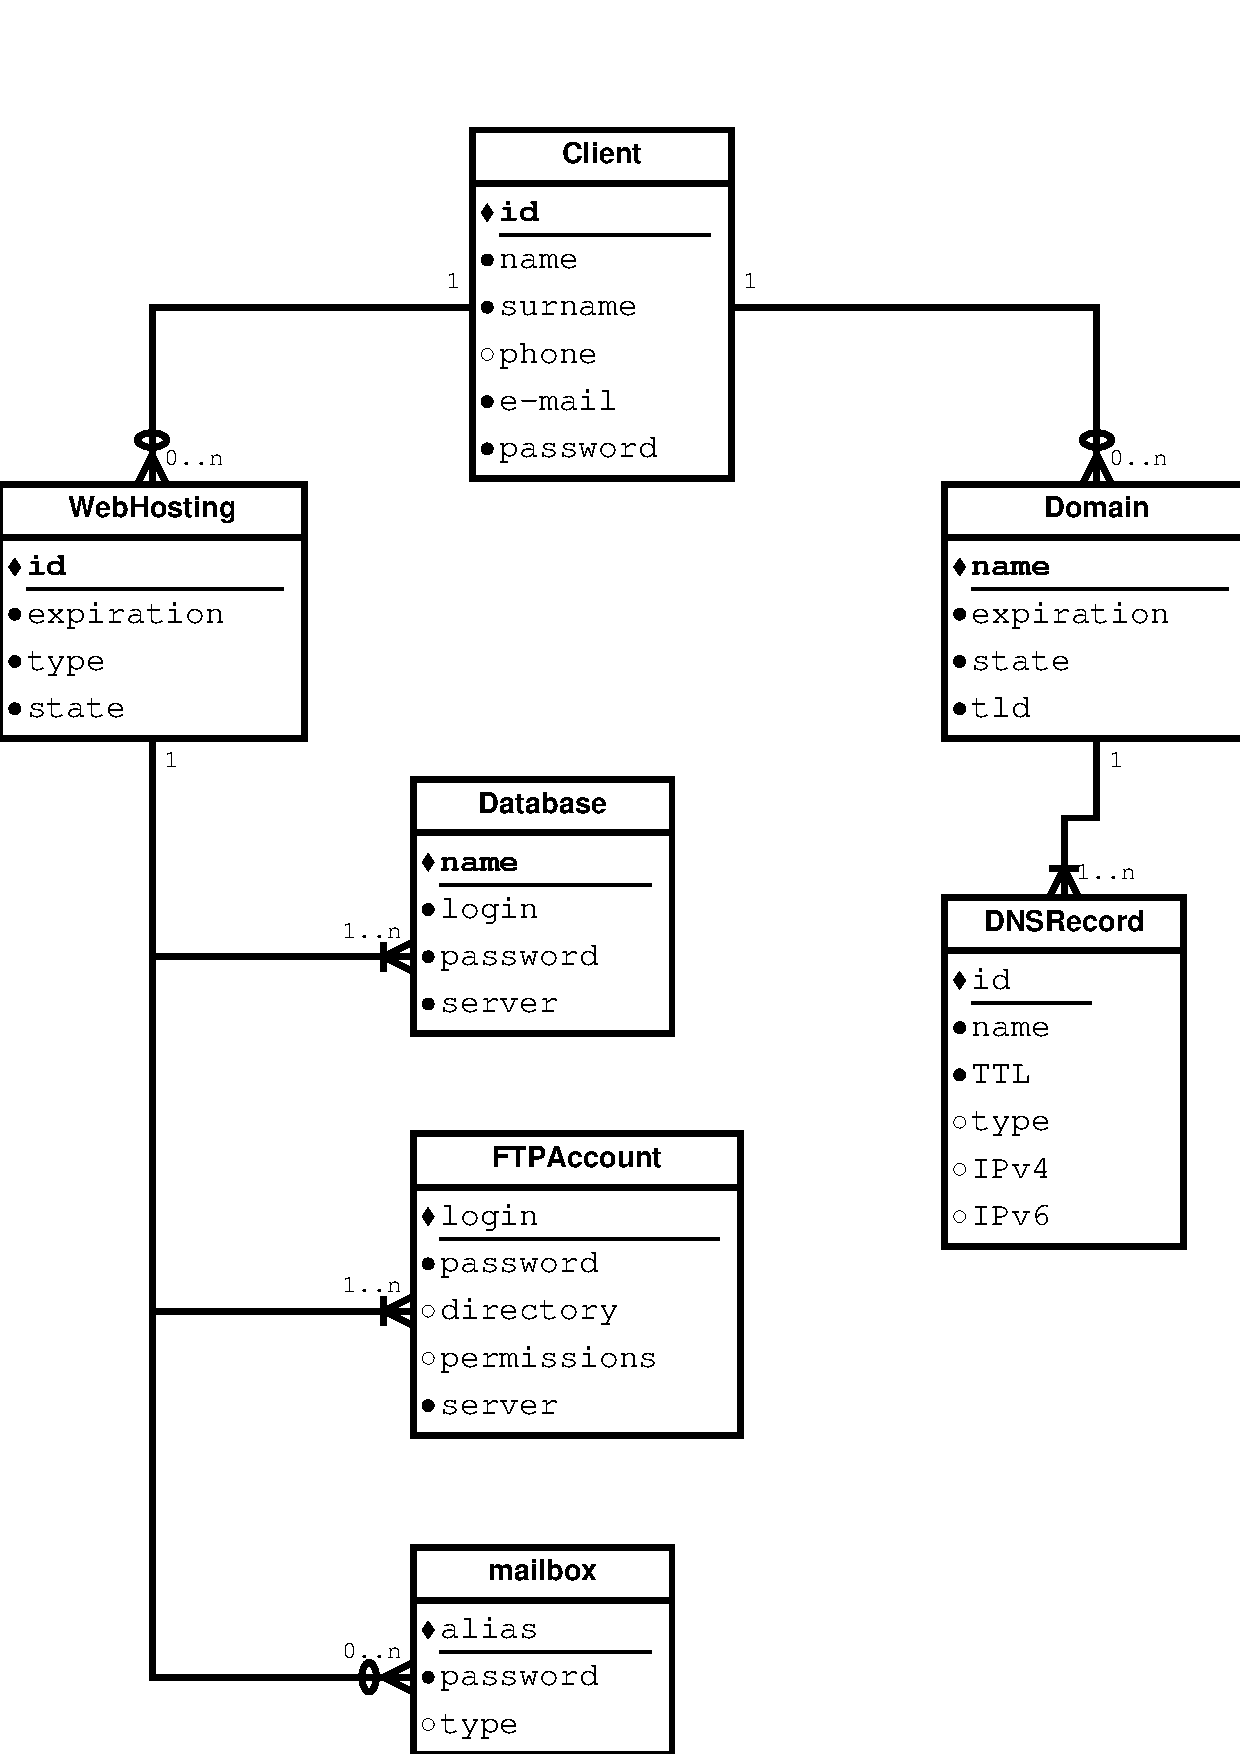
\includegraphics[width=10cm]{erd}
        \caption{ERD}
      \end{center}
    \end{figure}

\end{document}

